\documentclass[11pt,a4paper,titlepage, ngerman]{article}

\usepackage[utf8]{inputenc}	
\usepackage[T1]{fontenc}	
\usepackage{ngerman}			
\usepackage{lmodern}			
\usepackage{graphicx}			
\usepackage{url}				
\usepackage{siunitx}
\usepackage[intlimits]{amsmath}
\usepackage{xfrac}
\usepackage{commath}
\usepackage{physics}			
\usepackage{subcaption}
\usepackage{wrapfig}
\usepackage{biblatex}
\usepackage{hyperref}

% Setup SI unit environment
\sisetup{separate-uncertainty = true}
\sisetup{output-decimal-marker = {,}}
\sisetup{
	per-mode=fraction,
	fraction-function=\sfrac
	% or \frac, \tfrac
}
\bibliography{Literatur}
\begin{document}
	\begin{titlepage}
		\centering
		{\scshape\LARGE Versuchsbericht zu \par}
		\vspace{1cm}
		{\scshape\huge M4 -- Stoßgesetze\par}
		\vspace{2.5cm}
		{\LARGE Gruppe 10 Mi\par}
		\vspace{0.5cm}
		{\large Alex Oster (E-Mail: a\_oste16@uni--muenster.de) \par}
		{\large Jonathan Sigrist (E-Mail: j\_sigr01@uni--muenster.de) \par}
		\vfill
		durchgeführt am 13.12.2017\par
		betreut von\par
		{\large Semir \textsc{Vrana}} 
		\vfill	
		{\large \today\par}
	\end{titlepage}
	
	\tableofcontents
	
	\newpage
	
	\section{Kurzfassung}
	
	%TODO at the end kurzfassung{ziel, ergebnisse, wie gemacht}

	\vspace{2cm}	
	
	\section{Stoßprozess zweier Kugeln unterschiedlicher Masse}
	
	% Problem/Hypothese, Ansatz 
	Dieser Versuch dient zur Betrachtung der Stoßgesetze. Dazu wird ein ballistischer zentraler Stoß mit Hilfe von zwei aufgehängten Massen untersucht. Es stellt sich die Frage, wie genau die Stoßgesetze mit den gemessenen Werten übereinstimmen. Das Ergebnis dieser Messung zeigt, dass die Theorie mit den ermittelten Werten (nicht) übereinstimmt. % TODO 
	
	\subsection{Methoden}
		
		\subsubsection{Aufbau}
			
		Zum Messen verwenden wir den im Folgenden dargestellten Aufbau. Hierbei handelt es sich um zwei Pendel an denen Kugeln mit unterschiedlicher Masse angehängt sind. Die Schwerpunkte dieser Kugeln liegen auf einer Geraden, sodass ein ballistischer zentraler Stoß durch das Auslenken eines Pendels möglich ist. Für die Pendel wurden die Massen an Fäden gehängt, deren Enden jeweils auf gleicher Höhe befestigt wurden, so dass die Auslenkungen in einer Ebene stattfinden. Abbildung \ref{abb:VersuchsskizzeStoss} stellt dies dar. Dabei ist der Punkt in Ruhelage, wo die beiden Kugeln sich berühren durch $a_0$ gekennzeichnet. Des weiteren sind die Positionen der von $a_0$ gegenüber liegenden Punkte $a_1$ und $a_2$, welche um den Durchmesser der kleineren bzw. größeren Kugel, mit den Massen $m_1$ bzw. $m_2$, von $a_0$ verschieden sind, gekennzeichnet.
		\begin{figure}[ht]
			\centering
			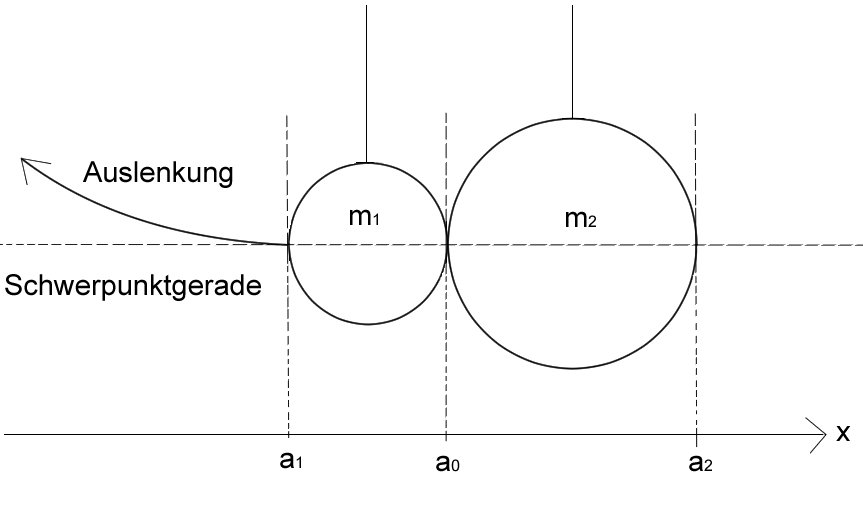
\includegraphics[width=\textwidth]{Kugelstoss.png}
			\caption{Skizzierung des Versuchsaufbaus}
			\label{abb:VersuchsskizzeStoss}	
		\end{figure}
		Dies wurde so gewählt, damit das Messen leichter fällt. Hierzu werden Schiebeblöcke verwendet (vgl. Abb. \ref{abb:VersuchsaufbauStoss}), welche sich auf einem Maß frei bewegen lassen. Damit sind $a_1'$ und $a_2'$ nach dem initialen Stoß leicht zu bestimmen. Die gestrichenen Variablen sollen hierbei die Auslenkung nach dem Stoß beschreiben. Zur Betrachtung im Schwerpunktsystem werden dann die Radien der Kugeln auf die Auslenkungen addiert bzw. subtrahiert (abhängig von der Seite). % TODO ?
		
		Es werden bei dem Versuch die Auslenkungen $a_1'$ und $a_2'$ für fünf verschiedene Startauslenkungen von $a_1$ und $a_2$ jeweils fünf mal gemessen, wobei die fünf Messwerte für dieselben Auslenkungen gemittelt werden.
		Zudem werden die Pendellänge und Masse der Kugeln bei beiden Pendeln gemessen. Ersteres mit Hilfe eines Maßbands und letzteres über eine Waage.	
		Über die Theorie des ballistischen zentralen Stoßes werden die Massen durch die anderen gemessenen Werte bestimmt und dann mit der gemessenen Masse verglichen. Dazu werden die Auslenkungen gegeneinander aufgetragen und das Verhältnis dabei bestimmt.
				
		\subsubsection{Unsicherheiten}
		
			Zur Berechnung der Unsicherheiten für die gemessenen und ermittelten Werte dient folgende Formel: 
			\begin{equation*}
				u(s) = \pm \sqrt{\sum_{k=0}^{N}\left( \frac{\partial f}{\partial x_i}u(x_i)\right) ^2}. \label{eq:kombUnsicherheit}
			\end{equation*}
			Für die von dem Maß(band) abgelesenen Werte werden Unsicherheiten über eine Dreiecksverteilung und für die von der Waage gemessenen Werte eine Rechteckverteilung verwendet. 
	
	\subsection{Messung}
	
		\subsubsection{Aufnahme der Messwerte}
		
			Für die Pendellängen wurden die Abstände zwischen den Schwerpunkten und den Befestigungshöhen gemessen. 
			Um die Radien der kugelförmigen Massen zu bestimmen, wurde der Umfang dieser gemessen. Die Werte der Pendellängen, der Radien, der gewogenen Massen und Startpunkte sind in Tabelle \ref{tab:Messwerte} dargestellt. Die Unsicherheit für die Radien steht in direktem Zusammenhang mit der Unsicherheit bei den Umfängen, also der des Maßbandes.
			\begin{table}[ht]
				\caption{Messwerte der Pendellänge, Masse und der Radien}
				\centering
				\label{tab:Messwerte}
				\begin{tabular}{c|l|l}
					{} & {Pendel 1} & {Pendel 2}	\\
					\hline
					{Pendellänge} & {$L_1 = \SI{185+-0,02}{\cm}$} & {$L_2 = \SI{189+-0,02}{\cm}$}	\\
					\hline
					{Kugelmasse} & {$m_1 = \SI{191,47+-0,003}{\g}$} & {$m_2 = \SI{510,21+-0,003}{\g}$}	\\	
					\hline
					{Kugelradien} & {$r_1 = \SI{1,83+-0,003}{\cm}$} & {$r_2 = \SI{2,55+-0,003}{\cm}$}	\\			
				\end{tabular}
			\end{table}
			
			Wie in Abb. \ref{abb:VersuchsskizzeStoss} eingezeichnet, beschreiben $a_0$, $a_1$ und $a_2$  die Positionen zu Beginn der Messung. Im Laborbuch sind jedoch nur die Positionen über dem Maß nach der Auslenkung notiert, jedoch nicht die Auslenkungen selber. Zur Bestimmung dieser für beide Massen wird die Differenz zwischen den Startwerten und den gemittelten Messwerten gebildet. Die dadurch ermittelten Werte sind in Tabelle \ref{tab:Messwerte2} zu finden. Dabei ergeben sich die Unsicherheiten durch die der Startwerte, beim differenzieren, sowie der bei dem Mitteln entstandenen kombinierten Unsicherheit, welche sich aus fünf mal der Unsicherheit des Maßes, sowie einer zusätzlichen Unsicherheit für das nach Augenmaß durchgeführte Schieben der Blöcke von \SI{0,05}{\cm} ergibt. Für die Auslenkungen in der Tabelle bezeichnen $a_{1/2}^{*}$ die Startauslenkungen und $a_{1/2}'$ die Auslenkungen nach dem Stoß. 	
			\begin{table}[ht]
				\caption{Auslenkungen nach Stoß}
				\centering
				\label{tab:Messwerte2}
	
				\begin{tabular}{c|c|c}
					{$a_{1}^{*}$} & {$\bar{a_{1}}'$} & {$\bar{a_{2}}'$}	\\
					\hline
					{\SI{17,14+-0,03}{\cm}} & {\SI{6,66+-0,06}{\cm}} & {\SI{8,82+-0,06}{\cm}}\\
					{\SI{13,14+-0,03}{\cm}} & {\SI{5,6+-0,06}{\cm}} & {\SI{6,40+-0,06}{\cm}}\\
					{\SI{11,14+-0,03}{\cm}} & {\SI{4,76+-0,06}{\cm}} & {\SI{5,62+-0,06}{\cm}}\\
					{\SI{9,14+-0,03}{\cm}} & {\SI{3,78+-0,06}{\cm}} & {\SI{4,40+-0,06}{\cm}}\\
					{\SI{5,14+-0,03}{\cm}} & {\SI{2,3+-0,06}{\cm}} & {\SI{2,32+-0,06}{\cm}}\\		
					\hline 
					& & \\
					{$a_{2}^{*}$} & {$\bar{a_{1}}'$} & {$\bar{a_{2}}'$}	\\
					\hline
					{\SI{10,1+-0,03}{\cm}} & {\SI{14,62+-0,06}{\cm}} & {\SI{4,98+-0,06}{\cm}}\\
					{\SI{8,1+-0,03}{\cm}} & {\SI{11,74+-0,06}{\cm}} & {\SI{4,14+-0,06}{\cm}}\\
					{\SI{6,1+-0,03}{\cm}} & {\SI{9,04+-0,06}{\cm}} & {\SI{3,22+-0,06}{\cm}}\\
					{\SI{4,1+-0,03}{\cm}} & {\SI{6,04+-0,06}{\cm}} & {\SI{2,32+-0,06}{\cm}}\\
					{\SI{2,1+-0,03}{\cm}} & {\SI{3,36+-0,06}{\cm}} & {\SI{1,4+-0,06}{\cm}}\\	
				\end{tabular}	
			\end{table}
	
		\subsubsection{Datenanalyse}	
			
			Nach den Gesetzen der Impuls- und Energieerhaltung gilt für den Stoßgeraden der folgende Zusammenhang zwischen stoßender und gestoßener Kugel:
			\begin{equation}
				a_2' = \frac{2m_\text{1}}{m_\text{1}+m_\text{2}} \cdot a_1^{*}.
			\end{equation}
			Zu beachten ist, dass hierbei $m_1$ die Masse der stoßenden Kugel ist. Umgekehrt lassen sich die Indizes tauschen, um den Fall mit $m_2$ als Masse der stoßenden Kugel abzudecken. Es folgt ein linearer Zusammenhang zwischen $a_2'$ und $a_1^{*}$ mit dem Faktor $\frac{2m_\text{1}}{m_\text{1}+m_\text{2}}$ bzw. umgekehrt. Ein Wert für diese Steigung ergibt sich, wenn man die ermittelten Werte für $a_2'$ gegen die von $a_1^{*}$ oder andersherum aufträgt.
			\begin{figure}[ht]
				\centering
				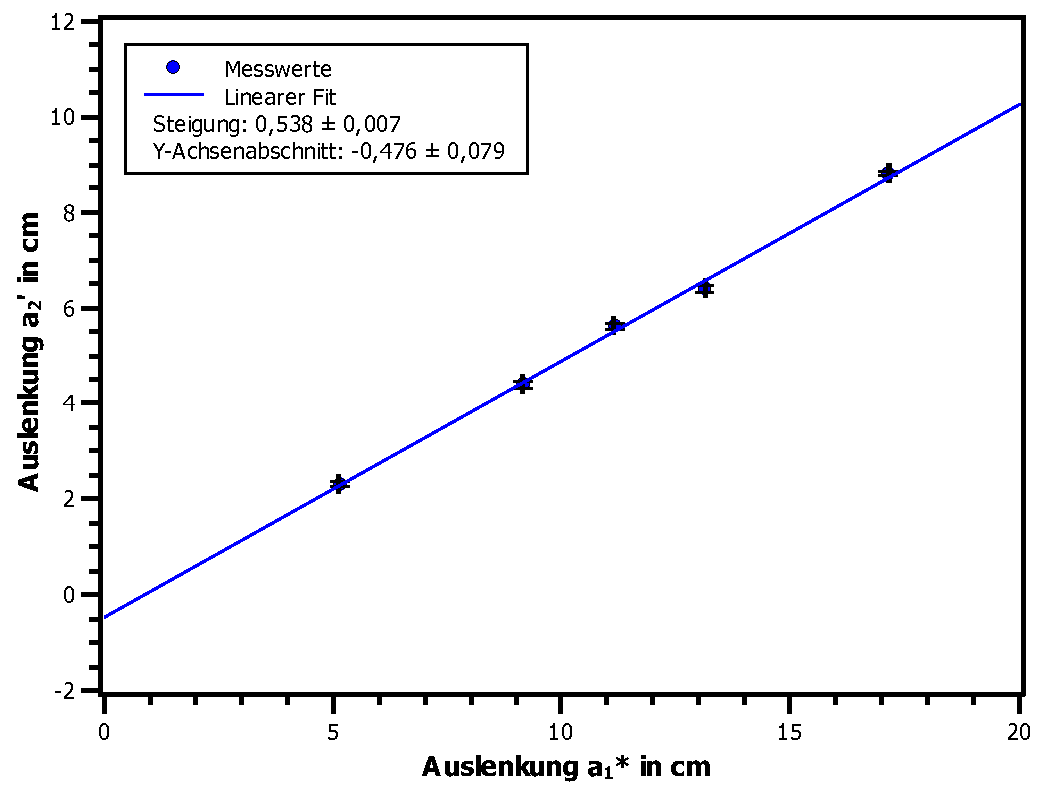
\includegraphics[width=\textwidth]{AuslenkungMittel.pdf}
				\caption{Auslenkung nach Stoß von $m_1$ auf $m_2$}
				\label{abb:AuslenkungMittel}	
			\end{figure}
			\begin{figure}[ht]
				\centering
				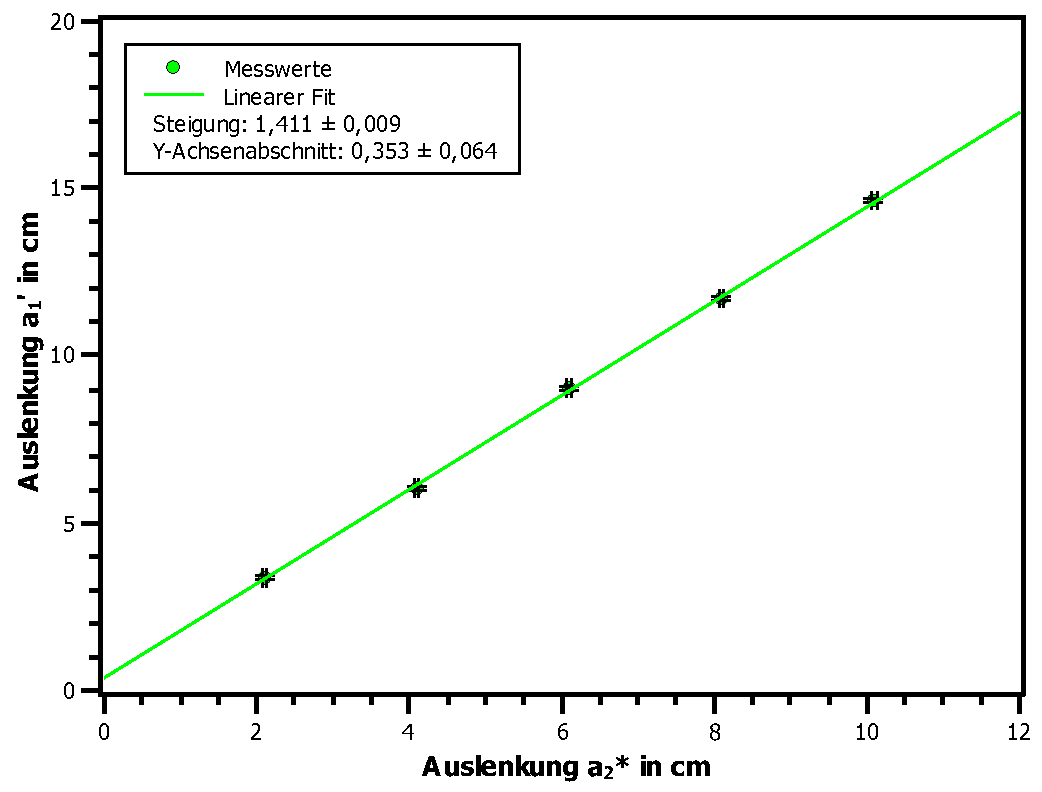
\includegraphics[width=\textwidth]{AuslenkungGross.pdf}
				\caption{Auslenkung nach Stoß von $m_2$ auf $m_1$}
				\label{abb:AuslenkungGross}	
			\end{figure}
			\footnote{Der Fit wurde von dem Programm SciDavis berechnet, dazu wurden die Unsicherheiten der Auslenkung und die Methode der kleinsten Quadrate herangezogen}
	\subsection{Diskussion}
	
	\subsection{Schlussfolgerung} %TODO Alex
	\newpage
	\section{Stoßprozesse mit einer Fallrinne}
Der Versuch stellt einen Zusammenhang zwischen der Höhenenergie einer kleinen Kugel und der Auslenkung eines Pendels nach einem Stoß her.
Dabei wird die kleine Metallkugel in einer Fallrinne bei verschiedenen Positionen losgelassen und der Energieübertrag bei dem Stoß mit der Pendelkugel untersucht.
Es wird der theoretische Anteil der kinetischen Energie mit $\varepsilon = \frac{5}{9}$ der Gesammtenergie überprüft und begründet, dass die Rollreibung des Systems diesen Anteil verfälscht.

	\subsection{Methoden}
	Die Fallrinne sei so justiert, dass die kleine Kugel der Rinne in einem geraden, zentralen Stoß auf die großen Kugel des Pendels trifft.
	Die große Kugel ruht dabei vor dem Stoß direkt am Ende der Fallrinne.
	Die kinetische Energie der kleinen Kugel wird bei dem Stoß an die große Kugel zu einem großen Teil übertragen.
	Nach dem Stoß wird die Auslenkung der großen Kugel abgelesen.
	
	In Abb. \ref{fig:fallrinneSkizze} kann man $s$ als Abstand vom oberen Rand der Fallrinne identifizieren.
	Es werden nun für die Abstände $s$ von \SIrange{0}{50}{\centi\meter}, jeweils in \SI{10}{\centi\meter}-Schritten mehrere Messungen der maximalen Auslenkung der großen Kugel nach dem Stoß durchgeführt.
	
	\begin{figure}[ht]
		\centering
		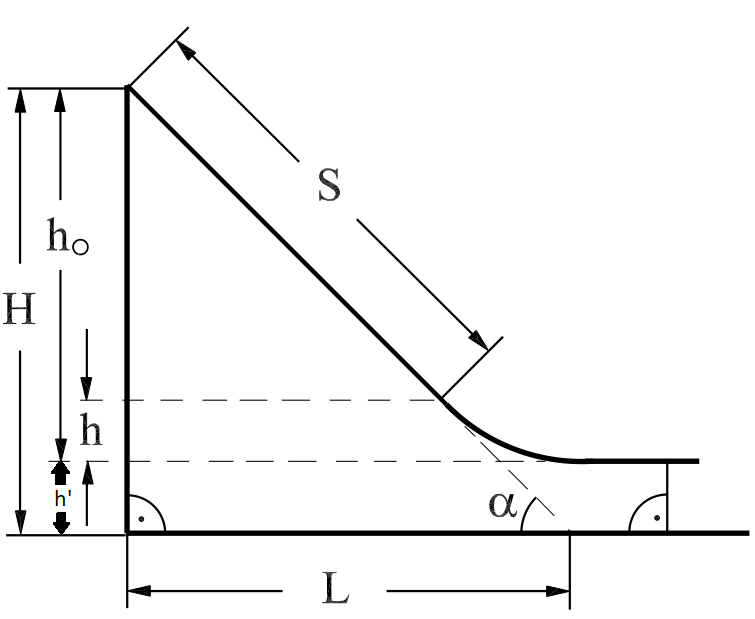
\includegraphics[width=0.6\textwidth]{FallrinneSkizze.png}
		\caption{Skizze der Fallrinne.}
		\label{fig:fallrinneSkizze}	
	\end{figure}

	\subsubsection*{Unsicherheiten}
	Die direkt gemessenen Größen seien mit den folgenden Unsicherheiten gemessen.
	
	Alle Längenmessungen wurden durch ein Maßstab oder -band gemacht, welches auf einen Millimeter genau abgelese nwerden konnte.
	Soweit nicht weiter aufgeführt, sei hier eine Unsicherheit von $u_0(l) = \frac{\SI{0,1}{\centi\meter}}{2\sqrt{6}} \approx \SI{0,02}{\centi\meter}$ anzunehmen.
	
	Für die Pendellänge wird durch erschwerte Ablesbarkeit an der Halterung eine Unsicherheit von $u(l) = \frac{\SI{1}{\centi\meter}}{2\sqrt{6}} \approx \SI{0,2}{\centi\meter}$ angenommen.
	Da die Halterungen für die beiden Seilenden des Pendels nicht optimal zentriert und auf leicht unterschiedlichen Höhen positioniert waren, konnte die Länge des Pendels von der Mitte der Halterung nicht Millimeter genau abgelesen werden.
	
 	Wie in Abb. \ref{fig:fallrinneSkizze} abgebildet, ist die Fallrinne zum Winkel $\alpha$ gerade weitergeführt worden, um einen Schnittpunkt mit der unteren Schiene zu bekommen.
	Durch diese Abschätzung ist die Unsicherheit für die Länge $L$ der Konstruktion mit $u(L) = \frac{\SI{0,5}{\centi\meter}}{2\sqrt{6}} \approx \SI{0,1}{\centi\meter}$ etwas höher gewählt.
	
	Die Waage hatte eine Unsicherheit von $u(m_1) = u(m_2) = \frac{\SI{0,01}{g}}{2\sqrt{3}} \approx \SI{0,003}{g}$.
	
	\subsection{Messung}
	
	Für die Abmessungen der Fallrinne wurde für $L = \SI{32,7 +- 0,1}{\centi\meter}$ gemessen.
	In Tab. \ref{tab:Messwerte} sind die Höhen über der untere Schiene der Fallrinne (vgl. Abb. \ref{fig:fallrinneSkizze}, Länge $L$) angegeben.
	\begin{table}[ht]
		\centering
		\caption{Höhenmessungen über der unteren Schiene und gemittelte Auslenkung des Pendels nach dem Stoß für die einzelnen Kugelpositionen.}
		\begin{tabular}{S|S|S}
			\hline
			{Abstand $s$} & {Höhe $H(s)$}  & {Auslenkung $a'_2$}\\
			\hline
			\SI{0 +- 0,1}{\centi\meter} & \SI{32,7 +- 0,1}{\centi\meter} & \SI{16,72 +- 0,24}{\centi\meter}\\
			\SI{10 +- 0,1}{\centi\meter} & \SI{27,2 +- 0,1}{\centi\meter} & \SI{15,30 +- 0,35}{\centi\meter}\\
			\SI{20 +- 0,1}{\centi\meter} & \SI{21,9 +- 0,1}{\centi\meter} & \SI{13,34 +- 0,11}{\centi\meter}\\
			\SI{30 +- 0,1}{\centi\meter} & \SI{16,7 +- 0,1}{\centi\meter} & \SI{11,52 +- 0,16}{\centi\meter}\\
			\SI{40 +- 0,1}{\centi\meter} & \SI{11,3 +- 0,1}{\centi\meter} & \SI{9,12 +- 0,15}{\centi\meter}\\
			\SI{50 +- 0,1}{\centi\meter} & \SI{5,7 +- 0,1}{\centi\meter} & \SI{5,94 +- 0,25}{\centi\meter}\\
			\hline
		\end{tabular}
	\end{table}
	Wir haben leider erst in der Auswertung gemerkt, dass wir die Grundhöhe der Rinne $H - h_0$ nicht gemessen haben.
	Deswegen muss diese Höhe dem $y$-Achsenabschnitt der Linearisierung entnommen werden.
	Aus diesem Grund wird die Analyse etwas anders durchgeführt.
	
	Für die kleine Kugel wurde ein Gewicht von \SI{63,69}{g}, für die große Kugel eines von \SI{510,21}{g} gemessen.
	
	\subsection{Datenanalyse}
	
	Die Fallhöhe der kleinen Kugel kann mit Abb. \ref{fig:fallrinneSkizze} hergeleitet werden.
	Es wird schnell deutlich, dass $h = h_0 - s \sin \alpha$ ist.
	Die beiden Größen $L$ und $H$ hängen mit $\tan \alpha = \frac{H}{L}$ zusammen.
	Stellt man diese etwas um, folgt
	\begin{equation}
		\frac{1}{\sin^2 \alpha} = 1 + \cot^2 \alpha = 1 + \frac{L^2}{H^2} \Leftrightarrow \sin \alpha = \frac{1}{\sqrt{1 + 	\frac{L^2}{H^2}}}.
	\end{equation}
	Oben eingesetzt ergibt sich 
	\begin{equation}
		\label{eq:hoehe}
		h = h_0 - \frac{s}{\sqrt{1 + \frac{L^2}{H^2}}}.
	\end{equation}
	Nach Gl. (28) der Einführung ist die maximale Auslenkung der großen Kugel gegeben durch
	\begin{equation}
		\label{eq:auslenkung}
		a'_2 = \frac{2 m_1}{m_1 + m_2} \sqrt{2 \varepsilon l h} \quad \text{mit} \quad \varepsilon = \frac{5}{9}.
	\end{equation}
	Setzt man nun Gl. (\ref{eq:hoehe}) in Gl. (\ref{eq:auslenkung}) ein und quadriert beide Seiten:
	\begin{equation}
		\label{eq:auslenkung2}
		(a'_2)^2 = \left( \frac{2 m_1}{m_1 + m_2}\right) ^2 2 \varepsilon l h = \varepsilon\gamma \left( h_0 - \frac{s}{\sqrt{1 + \frac{L^2}{H^2}}}\right),
	\end{equation}
	so ist $h_0$ von $s$ separiert und tritt als $y$-Achsenabschnitt einer linearen Gleichung nach $s$ auf\footnote{In der Anleitung soll $a'_2$ gegen $\sqrt{h}$ aufgetragen werden. Da wir einen Wert nicht mit aufgenommen hatten, ist die Linearisierung so deutlich einfacher und führt ebenso zum Ziel. Im späteren Verlauf wird der fehlende Wert aus der Linearisierung errechnet und auf Plausibilität geprüft.}.
	
	\begin{figure}[ht]
		\centering
		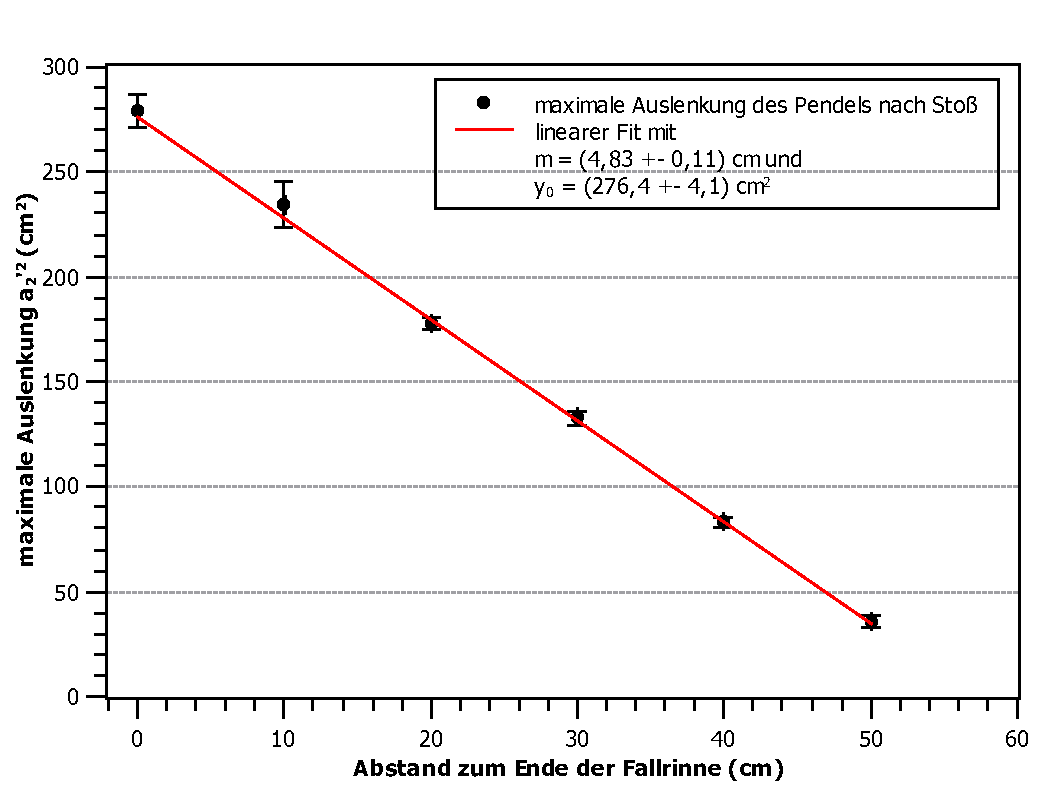
\includegraphics[width=\textwidth]{AuslenkungProAbstand.pdf}
		\caption{Maximale Auslenkung des Pendels bei unterschiedlichen Werten für $s$. Die Regressionsgerade zeigt den linearen Zusammenhang deutlich und liefert eine Steigung $m$, sowie einen $y$-Achsenabschnitt $y_0$.}
		\label{fig:fallrinneAuslenkung}	
	\end{figure}

	In Abb. \ref{fig:fallrinneAuslenkung} ist diese Linearisierung dargestellt.
	Nun wird der Anteil $\varepsilon$ der dem Stoß zur Verfügung stehenden Energie berechnet.
	Dazu wird aus Gl. (\ref{eq:auslenkung2}) die Steigung der Theorie mit der Steigung der Regressionsgeraden gleichgesetzt\footnote{Unsicherheitsrechnung im Anhang Gl. (\ref{eq:kombUnsicherheit}) mit Gl. (\ref{eq:epsilon}) bis Gl. (\ref{eq:epsilonEnd}).}:
	\begin{equation}
		m = -\frac{\varepsilon \gamma}{\sqrt{1 + \frac{L^2}{H^2}}} \Rightarrow \varepsilon = -\frac{m}{\gamma} \sqrt{1+\frac{L^2}{H^2}} \approx \SI{0,484 +- 0,012}{}.
	\end{equation}
	
	Zudem kann nun die fehlende Messung überprüft werden.
	Dazu wird aus Gl. (\ref{eq:auslenkung2}) für $s = 0$ der $y$-Achsenabschnitt der Ausgleichsgerade eingesetzt.
	Es folgt
	\begin{equation}
		\varepsilon \gamma h_0 = (a'_2)^2= y_0 \Rightarrow h_0 = \frac{y_0}{\varepsilon\gamma} \approx \SI{31,30 +- 0,88}{\centi\meter}
	\end{equation}
	und somit für die nicht gemessene Größe
	\begin{equation}
		h' = H - h_0 \approx \SI{1,40 +- 0,89}{\centi\meter}.
	\end{equation}
	
	\subsection{Schlussfolgerung}
	
	Der Versuch zeigt eine nicht unerhebliche Abweichung vom theoretisch hergeleiteten Faktor $\varepsilon = \frac{5}{9}$.
	Das könnte an der Reibung der Kugel auf der Fallrinne liegen, da die Kugel abgebremst wird und Energie verliert.
	Die Differenz von der potentiellen Höhenenergie am Anfang und bei maximaler Auslenkung ist also größer, als von der Theorieannahme und $\varepsilon$ der nutzbaren Energie somit kleiner.
	
	Die Nachrechnung der Höhe $h'$ ist damit auch nicht mehr genau.
	Mit dem theoretischen Wert von $\varepsilon = \frac{5}{9}$, ist $h' \approx \SI{5,4}{\centi\meter}$, also deutlich näher an der Realität.
	
	\subsection{Formeln}
	\begin{equation}
	\label{eq:unce_auslenkung2}
	u(a^2) = \pdv{a^2}{a} \cdot u(a) = 2 a \cdot u(a)
	\end{equation}
	
	\begin{align}
	\label{eq:epsilon}
	\varepsilon &= -\frac{m}{2 l} \left( \frac{m_1 + m_2}{2 m_1}\right) ^2 \sqrt{1+\frac{L^2}{H^2}}\\
	\pdv{\varepsilon}{m} &= \frac{\varepsilon}{m}\\
	\pdv{\varepsilon}{l} &= -\frac{\varepsilon}{l}\\
	\pdv{\varepsilon}{m_1} &= +\frac{m}{4 l} \sqrt{1+\frac{L^2}{H^2}} \cdot \frac{m_1 + m_2}{m_1} \cdot \frac{m_2}{m_1^2}\\
	\pdv{\varepsilon}{m_2} &= -\frac{m}{4 l} \sqrt{1+\frac{L^2}{H^2}} \frac{m_1 + m_2}{m_1} \frac{1}{m_1}\\
	\pdv{\varepsilon}{L} &= -\frac{m}{2 l} \left( \frac{m_1 + m_2}{2 m_1}\right) ^2 \frac{L}{H^2}\frac{1}{\sqrt{1+\frac{L^2}{H^2}}}\\
	\pdv{\varepsilon}{H} &= +\frac{m}{2 l} \left( \frac{m_1 + m_2}{2 m_1}\right) ^2 \frac{L^2}{H^3}\frac{1}{\sqrt{1+\frac{L^2}{H^2}}}
	\label{eq:epsilonEnd}
	\end{align}
	 %TODO Joey
	
	%\section*{Literatur}
	%\printbibliography
	
	\newpage
	
	\section{Anhang}
	
	%TODO einfach einfuegen
	
	\begin{figure}[ht]
		\centering
		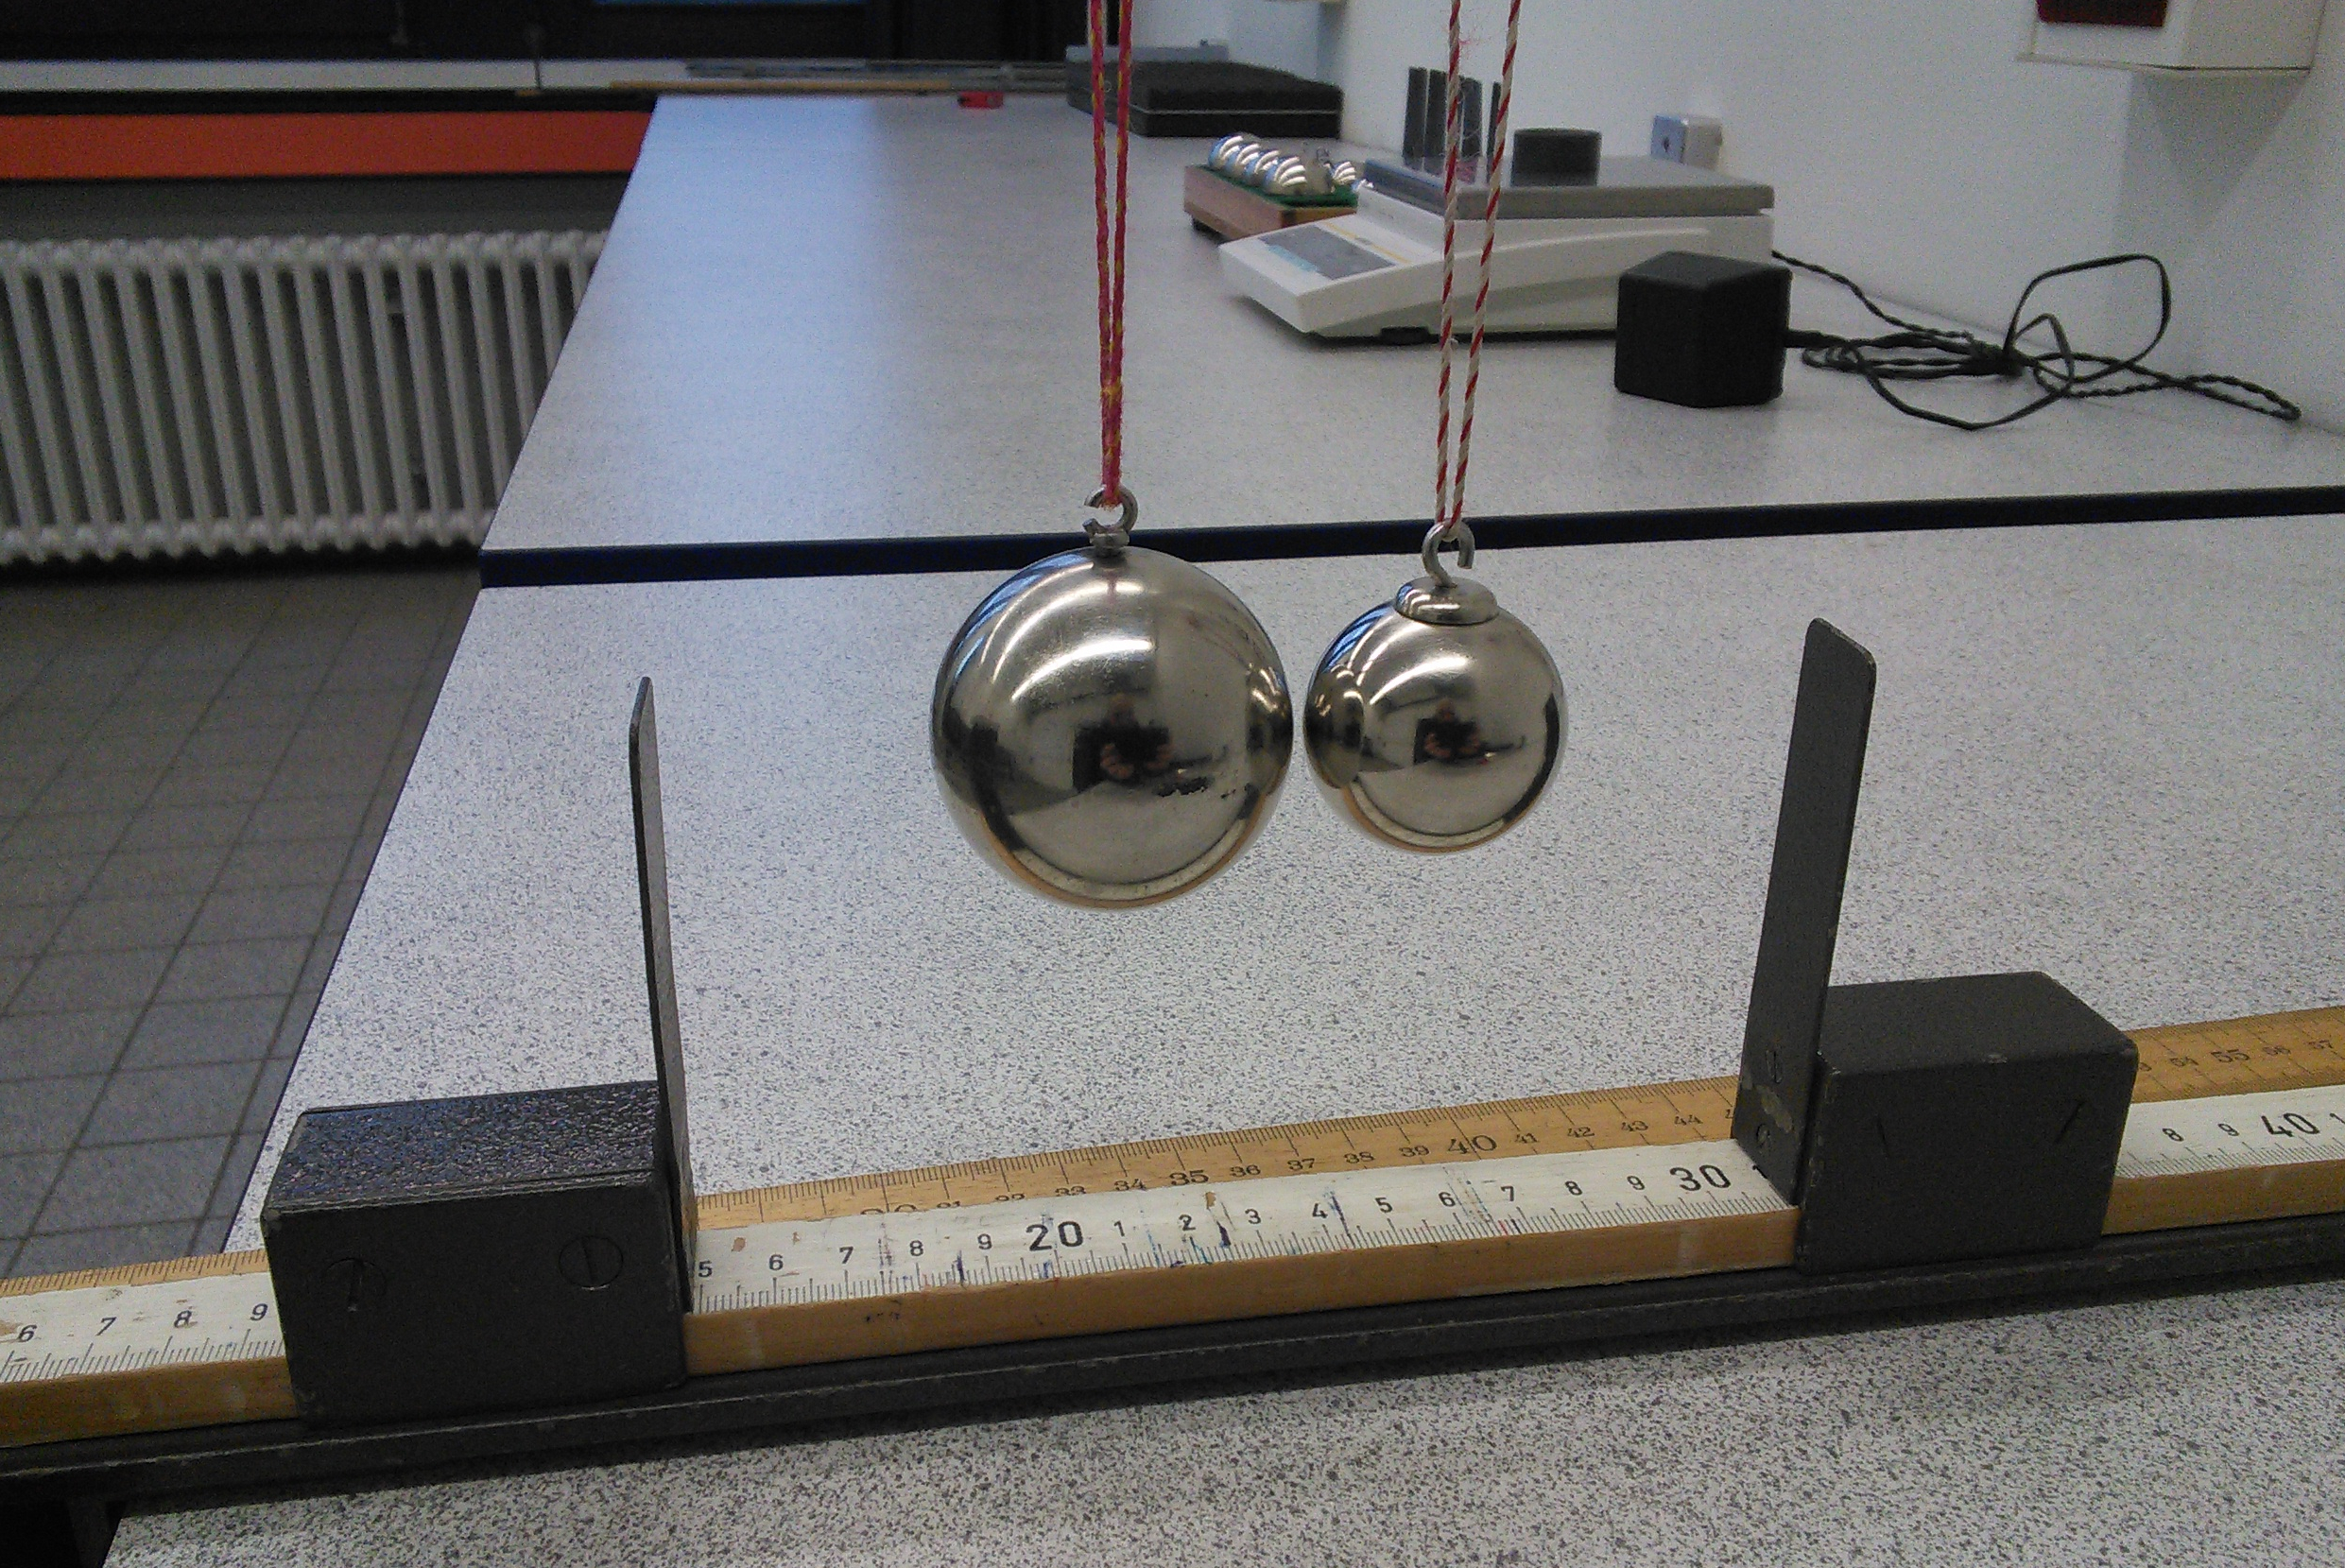
\includegraphics[width=\textwidth]{M4_1.jpg}
		\caption{Versuchsaufbau$^{[1]}$}
		\label{abb:VersuchsaufbauStoss}	
	\end{figure}
	
	\section*{Literatur}
	
	%TODO einfach einfuegen
	
	[1] Abb. \ref*{abb:VersuchsaufbauStoss} stammt aus der Vorbereitung zu M4, welche im Learnweb zu finden ist.
	
\end{document} 